\documentclass[t, handout]{beamer}
\usepackage[utf8]{inputenc} %extra characters
\usepackage[ngerman]{babel} %deutsche Spracheinstellung
\usepackage{blindtext} %generiert zufälligen Text
\usepackage{amsmath,amssymb} % erleichtert Mathe 
\usepackage{enumerate} % schicke Nummerierung
%\usepackage{enumitem} %römische/alphabetische Nummerierung
\usepackage{graphicx} % für Grafik-Einbindung
\usepackage{framed}
\usepackage{xcolor}
\usepackage{mdframed}
\usepackage{hyperref}
\usepackage[backend=biber,style=numeric,]{biblatex}
\hypersetup{
colorlinks=true, %set true if you want colored links
linktoc=all,        %set to all if you want both sections and subsections linked
linkcolor=blue,   %choose some color if you want links to stand out
citecolor=blue,	%choose chite color
urlcolor = blue	%url color
}
\addbibresource{Literatur.bib}

\usepackage{caption}
\usepackage[rightcaption]{sidecap}
\captionsetup[figure]{format=plain,font=small,justification=raggedright}
%%%%%%%%%%%%%%%%%%%%%%%%%%%%%%%%%%%%%%%%%%%%%%%%%%%%%%%%%%%%%%%%%%
%
% shortcuts
%
\DeclareMathOperator{\GL}{GL} % einige Macro, siehe am Ende Abschn. 2
\newcommand{\N}{\mathbb{N}}
\newcommand{\Z}{\mathbb{Z}}
\newcommand{\Q}{\mathbb{Q}}
\newcommand{\R}{\mathbb{R}}
\newcommand{\C}{\mathbb{C}}
\newcommand{\cP}{{\mathcal P}} 
\newcommand{\K}{\mathbb{K}}
\newcommand{\RM}[1]{\MakeUppercase{\romannumeral #1{.}}} %römische Zahlen
%
% Ende shortcuts
%
%%%%%%%%%%%%%%%%%%%%%%%%%%%%%%%%%%%%%%%%%%%%%%%%%%%%%%%%%%%%%%%%%%
%Style
\mode<presentation>{
%Theme
%\usetheme{default}
%\usetheme{AnnArbor}
%\usetheme{Antibes}
%\usetheme{Bergen}
%\usetheme{Berkeley}
%\usetheme{Berlin}
%\usetheme{Boadilla}
%\usetheme{CambridgeUS}
%\usetheme{Copenhagen}
%\usetheme{Darmstadt}
%\usetheme{Dresden}
%\usetheme{Frankfurt}
%\usetheme{Goettingen}
%\usetheme{Hannover}
%\usetheme{Ilmenau}
%\usetheme{JuanLesPins}
%\usetheme{Luebeck}
\usetheme{Madrid}
%\usetheme{Malmoe}
%\usetheme{Marburg}
%\usetheme{Montpellier}
%\usetheme{PaloAlto}
%\usetheme{Pittsburgh}
%\usetheme{Rochester}
%\usetheme{Singapore}
%\usetheme{Szeged}
%\usetheme{Warsaw}

%Farb-Theme
%\usecolortheme{albatross}
%\usecolortheme{beaver}
%\usecolortheme{beetle}
%\usecolortheme{crane}
%\usecolortheme{dolphin}
%\usecolortheme{dove}
%\usecolortheme{fly}
%\usecolortheme{lily}
%\usecolortheme{orchid}
\usecolortheme{rose}
%\usecolortheme{seagull}
%\usecolortheme{seahorse}
%\usecolortheme{whale}
%\usecolortheme{wolverine}

%\setbeamertemplate{footline} % Fußzeile entfernen
\setbeamertemplate{footline}[page number] % Fußzeile entfernen und durch Folien-Zahl ersetzen
\setbeamertemplate{navigation symbols}{} % Navigations-Symbole entfernen
\setbeamertemplate{theorems}[numbered]

}
%%%%%%%%%%%%%%%%%%%%%%%%%%%%%%%%%%%%%%%%%%%%%%%%%%%%%%%%%%%%%%%%%%
\theoremstyle{definition} % insert bellow all blocks you want in italic
\newtheorem{sa}{Satz}[section] % to number according to section
\newtheorem{dfi}[sa]{Definition} % to number according to section
\newtheorem{lem}[sa]{Lemma}
\newtheorem*{idea}{Idee} % no numbered block
\newtheorem*{prob}{Problem}
\newtheorem*{bsp}{Beispiel}
\newtheorem{fol}[sa]{Folgerung}
%%%%%%%%%%%%%%%%%%%%%%%%%%%%%%%%%%%%%%%%%%%%%%%%%%%%%%%%%%%%%%%%%%

\title[Ailurus fulgens]{Banachräume}
\subtitle{Mathematisches Seminar\\ Wintersemester 2022}
\author{Patrick Müller}
\institute[LT]{Fakultät Angewandte Natur- und Geisteswissenschaften}
\date{25. Oktober 2022}
\titlegraphic{
\includegraphics[width=0.3\textwidth]{pictures/thws.png}}

%%%%%%%%%%%%%%%%%%%%%%%%%%%%%%%%%%%%%%%%%%%%%%%%%%%%%%%%%%%%%%%%%%
%Begin Document
%%%%%%%%%%%%%%%%%%%%%%%%%%%%%%%%%%%%%%%%%%%%%%%%%%%%%%%%%%%%%%%%%%
\begin{document}
\renewcommand{\figurename}{Abb.}

%Titelseite
\begin{frame}
\titlepage
\vspace{5pt}
{\centering \scriptsize{Prof. Dr. Michael Bodewig\\Prof. Dr. Christian Zirkelbach} \par}
\end{frame}
%Inhaltsverzeichnis
\begin{frame}
\frametitle{Inhalt}
\tableofcontents
\end{frame}

%Stefan Banach Bild
\begin{frame}
\frametitle{Stefan Banach}
\centering
\begin{figure}
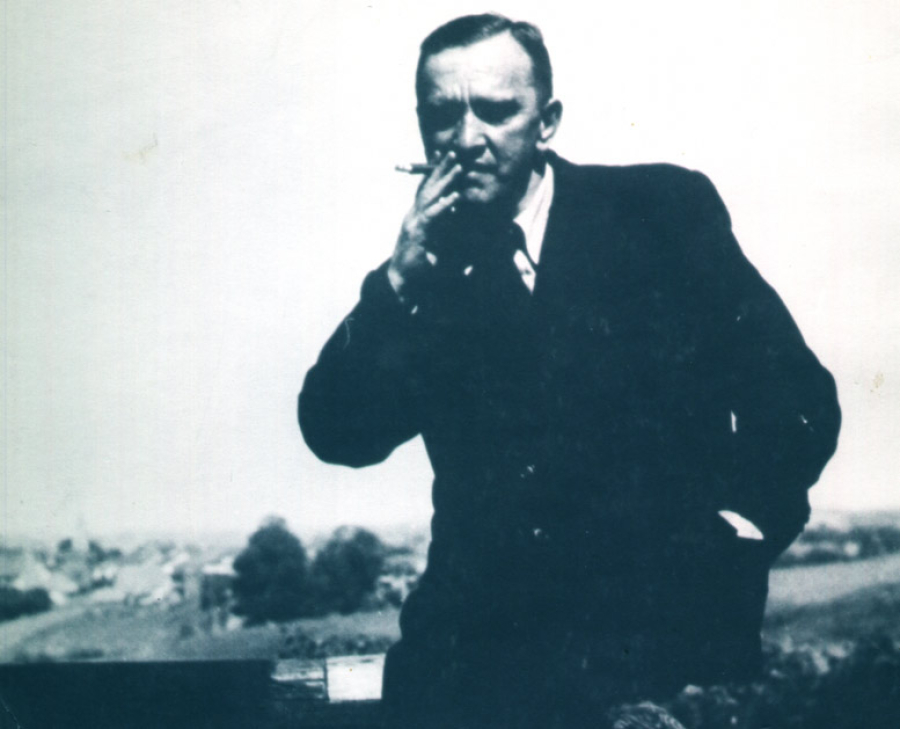
\includegraphics[width=0.75\textwidth]{pictures/stefan-banach.jpg}
\caption{Stefan Banach beim Chillen \cite{StefanBanach}}
\end{figure}
\end{frame}
%%%%%%%%%%%%%%%%%%%%%%%%%%%%%%%%%%%%%%%%%%%%%%%%%%%%%%%%%%%%%%%%%%
%Grundlagen
%%%%%%%%%%%%%%%%%%%%%%%%%%%%%%%%%%%%%%%%%%%%%%%%%%%%%%%%%%%%%%%%%%
\section{Grundlagen}

%%%%%%%%%%%%%%%%%%%%%%%%%%%%%%%%%
%Vektorraum
%%%%%%%%%%%%%%%%%%%%%%%%%%%%%%%%%
\subsection{Vektorraum}

\begin{frame}
\frametitle{Vektorraum}
\begin{block}{Wiederholung}
Ein Vektorraum $X$ über einem Körper $\K$ ist eine nichtleere Menge, die abgeschlossen ist bezüglich der Addition von Elementen aus $X$ (den Vektoren) und Multiplikation mit Elementen aus $\K$ (den Skalaren) sowie Assoziativ- und Distributivgesetze erfüllt sind.
\end{block}
\end{frame}

%%%%%%%%%%%%%%%%%%%%%%%%%%%%%%%%%
%Metrische Räume
%%%%%%%%%%%%%%%%%%%%%%%%%%%%%%%%%
\subsection{Metrische Räume}

\begin{frame}
\frametitle{Metrische Räume}
\begin{block}{Hinweis}
Wir interessieren uns für normierte Räume, doch viele Aussagen gelten auch allgemeiner auf metrischen Räumen. Auf diese Eigenschaft wollen wir nicht verzichten.
\end{block}
\begin{figure}
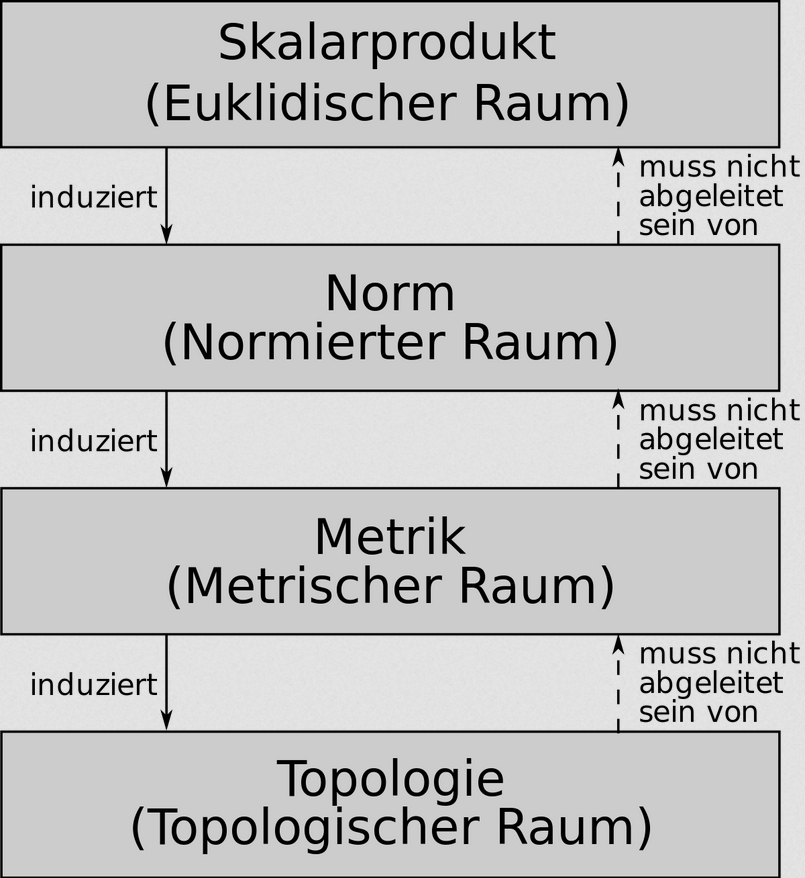
\includegraphics[width=0.37\textwidth]{pictures/hirarchie.png}
\caption{Hierarchie mathematischer Räume \cite{Hirarchie}}
\end{figure}
\end{frame}

\begin{frame}
\frametitle{Metrische Räume}
\begin{dfi}
(vgl. Ref. \cite{Forster}, Definition S.3): Sei $X$ eine Menge.  Eine \textit{Metrik} auf $X$ ist eine Abbildung $d : X \times X \rightarrow {\R_0}^+$, die für alle $x, y, z \in X$ die folgenden Eigenschaften erfüllt:
\begin{itemize}
\item[(i)] $d(x, y) = 0 \Leftrightarrow x = y$ (Nichtdegeneriertheit)
\item[(ii)] $d(x, y) = d(y, x)$ (Symmetrie)
\item[(iii)] $d(x, z) \leq d(x, y) + d(y, z)$ (Dreiecksungleichung)
\end{itemize}
Das Paar $(X, d)$ einen \textit{metrischen Raum}, wobei $d(x,y)$ einen Abstand zwischen den zwei Punkten $x$ und $y$ definiert.
\end{dfi}
\end{frame}

%%%%%%%%%%%%%%%%%%%%%%%%%%%%%%%%%
%Normierte Räume
%%%%%%%%%%%%%%%%%%%%%%%%%%%%%%%%%
\subsection{Normierte Räume}

\begin{frame}
\frametitle{Normierte Räume}
\begin{dfi}
(vgl. Ref. \cite{Werner}, Definition \RM{1}1.1):
Eine \textit{Norm} ist eine Abbildung 
\begin{align*}
 & {\|\cdot\|} : X \rightarrow {\R_0}^+, x \mapsto \|x\|
\end{align*}
von einem $\K$-Vektorraum $X$ in die nicht negativen reellen Zahlen ${\R_0}^+ := [0, \infty)$, die für alle $x, y \in X$ und $\lambda \in \K$ folgende Eigenschaften erfüllt:
\begin{itemize}
\item[(i)] ${\|x\|} = 0 \Leftrightarrow x = 0 \in X$ \textit{(Nichtdegeneriertheit)}
\item[(ii)] ${\|\lambda x\|} = |\lambda|{\|x\|}$ \textit{(Homogenität)}
\item[(iii)] ${\|x + y\|} \leq {\|x\|} + {\|y\|}$ \textit{(Dreiecksungleichung)}
\end{itemize}
\end{dfi}
\pause
Das Paar $(X , {\|\cdot\|})$ ist ein normierter Vektorraum. \\Wenn klar ist, welche Norm benutz wird, schreiben wir dafür kurz $X$.
\end{frame}

\begin{frame}
\frametitle{Normierte Räume}
\begin{bsp}
Wir definieren für $x \in X$ und Funktionen $f : D \subset X \rightarrow \R$ die Normen:
\begin{align*}
& \text{Summennorm:} \: {\|x\|}_1 := |x_1| + |x_2| + \cdots + |x_n| = \sum_{i=1}^n{|x_i|}\\
& \text{Maximumsnorm:} \: {\|x\|}_\infty := \max{(|x_1|, |x_2|, \cdots |x_n|)}\\
& \text{Supremumsnorm:} \: {\|f\|}_\infty := \sup_{x \in D}{|f(x)|}\\
& \text{Euklidische Norm:} \: {\|x\|}_2 := \sqrt{\sum_{i=1}^n{|x_i|^2}}\\
& \text{p-Norm:} \: {\|x\|}_p := \left(\sum_{i=1}^n{|x_i|^p}\right)^{1 \over p} \: \text{für} \: p \geq 1
\end{align*}
\end{bsp}
\end{frame}

%%%%%%%%%%%%%%%%%%%%%%%%%%%%%%%%%%%%%%%%%%%%%%%%%%%%%%%%%%%%%%%%%%
%Banachräume
%%%%%%%%%%%%%%%%%%%%%%%%%%%%%%%%%%%%%%%%%%%%%%%%%%%%%%%%%%%%%%%%%%
\section{Banachräume}
%%%%%%%%%%%%%%%%%%%%%%%%%%%%%%%%%
%Konvergenz in normierten Räumen
%%%%%%%%%%%%%%%%%%%%%%%%%%%%%%%%%
\subsection{Konvergenz in normierten Räumen}

\begin{frame}
\frametitle{Konvergenz in normierten Räumen}
\begin{dfi}
\label{konv}
Sie ${(x_k)}_{k \in \N} = (x_1, x_2, x_3, . . .)$ eine Folge aus Elementen $x_k \in X$ des Vektorraums, dann \textit{konvergiert} diese gegen $x \in X$, wenn gilt:
\begin{align*}
& \|x - x_k\| \rightarrow 0 \enspace \text{für} \enspace k \rightarrow \infty
\end{align*}
\end{dfi}
\pause
Man schreibt dann $x_k \rightarrow x$ für $k \rightarrow \infty$ oder $\lim\limits_{n \to \infty}{x_k} = x$.
\pause
\begin{dfi}[Epsilon-Schreibweise]
\label{konv_eps}
 Die Folge ${(x_k)}_{k \in \N}$ konvergiert gegen $x \in X$, wenn gilt:
\begin{align*}
& \forall \epsilon > 0 \enspace \exists N \in \N : \|x - x_k\| \leq \epsilon \enspace \text{für alle} \enspace k \geq N
\end{align*}
\end{dfi}
\end{frame}

\begin{frame}
\frametitle{Konvergenz in normierten Räumen}
\begin{prob}
Wir müssen in der Lage sein, ein $x \in X$ zu erraten, um die Definition \hyperref[konv]{\ref*{konv}} oder \hyperref[konv_eps]{\ref*{konv_eps}} zu benutzen.
\end{prob}
\pause
\begin{dfi}
\label{konv_cau}
Eine Folge ${(x_k)}_{k \in \N}$ in X ist eine \textit{Cauchy-Folge}, wenn gilt:
\begin{align*}
& \forall \epsilon > 0 \enspace \exists N \in \N : \|x_k - x_l\| \leq \epsilon \enspace \text{für alle} \enspace k,l \geq N
\end{align*}
\end{dfi}
\end{frame}

\begin{frame}
\frametitle{Konvergenz in normierten Räumen}
\begin{lem}
Jede konvergente Folge ist eine Cauchy-Folge.
\end{lem}
\pause
\begin{block}{Frage}
Ist mit dem Lemma  \hyperref[konv_cau]{\ref*{konv_cau}} unser Problem gelöst?
\end{block}
\pause
\begin{block}{Antwort}
Nein, leider nicht. :( Die "problematische" Definition \hyperref[konv]{\ref*{konv}} oder \hyperref[konv_eps]{\ref*{konv_eps}} erfüllt Definition \hyperref[konv_cau]{\ref*{konv_cau}}, jedoch nicht umgekehrt.
\end{block}
\pause
\begin{block}{Gute Nachricht}
In sehr vielen Räumen gilt auch die Umkehrung, also: Jede Cauchy-Folge ist konvergent. :)
\end{block}
\end{frame}

%%%%%%%%%%%%%%%%%%%%%%%%%%%%%%%%%
%Vollständigkeit
%%%%%%%%%%%%%%%%%%%%%%%%%%%%%%%%%
\subsection{Vollständigkeit}

\begin{frame}
\frametitle{Vollständigkeit}
\begin{dfi}
(vgl. Ref. \cite{Werner}, S.472) Ein Raum heißt vollständig, wenn in ihm jede Cauchy-Folge konvergiert.
\end{dfi}
\pause
\textit{Beispiel ...}
\pause
\begin{sa}
Jeder Raum $X$ kann vervollständigt werden. Es gibt einen vollständigen Raum $\hat{X}$ mit einer Isometrie $\varphi : X \rightarrow \hat{X}$, so dass $\varphi(X)$ dicht in $\hat{X}$ liegt. Der Raum $\hat{X}$ heißt \textit{Vervollständigung} von $X$.
\end{sa}
\pause
\begin{dfi}
(vgl. Ref. \cite{Alt}, S.28) Ein normierter Vektorraum $X$ heißt \textit{Banachraum}, wenn er vollständig (bezüglich der induzierten Metrik) ist.
\end{dfi}
\end{frame}

\begin{frame}
\frametitle{Vollständigkeit}
\begin{block}{Lösung}
Wir beschränken uns auf Banachräume
\end{block}
\pause
\begin{block}{Noch eine gute Nachricht}
Die meisten Räume, mit denen man sich in der angewandten Mathematik beschäftigt, sind Banachräume.
\end{block}
\end{frame}

\begin{frame}
\frametitle{Vollständigkeit}
\begin{sa}
(vgl. Ref. \cite{Clason}, Satz 3.8) Ist $E$ ein endlichdimensionaler Vektorraum, so sind alle Normen auf $E$ äquivalent.
\end{sa}
\pause
Vollständigkeit bleibt beim Übergang zu äquivalenten Normen erhalten. \newline Da $(E,\|\cdot\|_2)$ vollständig ist, können wir folgern:
\pause
\begin{fol}
(Ref. \cite{Clason}, Folgerung 3.9) Alle endlichdimensionalen normierten Vektorräume sind vollständig und somit Banachräume.
\end{fol}
\pause
\begin{fol}
(Ref. \cite{Clason}, Folgerung 3.4) Sind ${\|\cdot\|}_1$ und ${\|\cdot\|}_2$ äquivalente Normen auf $X$ , dann ist $(X , {\|\cdot\|}_1)$ ein Banachraum genau dann, wenn $(X , {\|\cdot\|}_2)$ ein Banachraum ist.
\end{fol}
\end{frame}

%%%%%%%%%%%%%%%%%%%%%%%%%%%%%%%%%
%Abgeschlossenheit
%%%%%%%%%%%%%%%%%%%%%%%%%%%%%%%%%
\subsection{Abgeschlossenheit}

\begin{frame}
\frametitle{Abgeschlossenheit}
Im folgenden sei $(X, d)$ ein metrischer Raum.
\pause
\begin{dfi}
Wir definieren für $x \in X$ und $r >0$
\begin{itemize}
\item[(i)] die \textit{offene Kugel} $U_r (x) := \{y \in X : d(x, y) < r \}$ 
\item[(ii)] die \textit{abgeschlossene Kugel} $B_r (x) := \{y \in X : d(x, y) \leq r \}$ 
\end{itemize}
um den Punkt $x$ mit Radius $r$.
\end{dfi}
\pause
\begin{dfi}[offene Menge]
Eine Menge $O \subset X$ heißt \textit{offen}, wenn jedes Element $x \in O$ ein innerer Punkt von $O$ ist.
\end{dfi}
\pause
\begin{dfi}[offene Menge - Epsilon-Schreibweise]
Eine Menge $O \subset X$ heißt offen, wenn gilt:
\begin{align*}
 \forall x \in O \enspace \exists \epsilon > 0 : U_\epsilon(x) \subset O
\end{align*}
\end{dfi}
\end{frame}

\begin{frame}
\frametitle{Abgeschlossenheit}
\begin{dfi}[abgeschlossene Menge]
Eine Menge $A \subset X$ heißt \textit{abgeschlossen}, wenn die Menge $X \setminus A$ offen ist.
\end{dfi}
\pause
\begin{dfi}[beschränkte Menge]
$A \subset X$ heißt \textit{beschränkt}, falls sie einen endlichen Durchmesser besitzt:
\begin{align*}
\text{diam}(A) = \sup_{x,y \in A}{d(x,y)} < \infty
\end{align*}
\end{dfi}
\pause
\centering
\begin{figure}
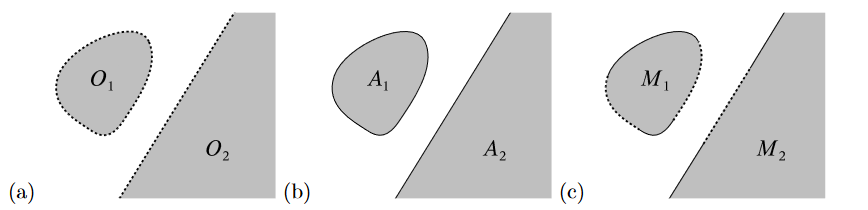
\includegraphics[width=0.85\textwidth]{pictures/offene-abgeschlossene-mengen.png}
\caption{(a) offene Teilmengen in $\R^2$. (b) abgeschlossene Teilmengen in $\R^2$. \newline(c) Teilmengen des $\R^2$, welche weder offen noch abgeschlossen sind. \cite{OffeneAbgeschlosseneMengen}}
\end{figure}
\end{frame}

\begin{frame}
\frametitle{Abgeschlossenheit}
\begin{dfi}
Für $M \subset X$ definieren wir:
\begin{itemize}
\item[(i)] das \textit{Innere} $M^\circ = M \setminus \partial M$
\item[(ii)] den \textit{Abschluss} $\bar{M} = M \cup \partial M$
\end{itemize}
\end{dfi}
\pause
\centering
\begin{figure}
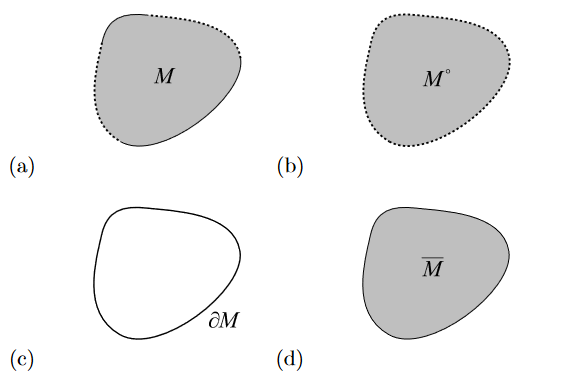
\includegraphics[width=0.5\textwidth]{pictures/innerer-abschluss.png}
\caption{(a) eine Teilmenge $M$ des $\R^2$. (b) das Innere von $M$. (c) der Rand von $M$. (d) der Abschluss von $M$. \cite{OffeneAbgeschlosseneMengen}}
\end{figure}
\end{frame}


\begin{frame}
\frametitle{Abgeschlossenheit}
\begin{sa}[Folgenkriterium für Abgeschlossenheit]
Eine Teilmenge $A \subset X$ ist genau dann abgeschlossen, wenn der Grenzwert jeder konvergenten Folge in $A$ ein Element von $A$ ist.
\end{sa}
\pause
Damit kann man oft die Abgeschlossenheit einer Menge widerlegen.
\pause
\textit{Beispiel ...}
\pause
\begin{block}{Wiederholung}
Ein Unterraum ist eine Teilmenge, die abgeschlossen bezüglich der Vektorraumoperationen ist.
\end{block}
\pause
\begin{sa}
\label{abgeschlossenerUnterraum}
(Ref. \cite{Clason}, Lemma 3.5) Sei $(X , {\|\cdot\|})$ ein Banachraum und $U \subset X$ ein Unterraum. Dann ist $(U , {\|\cdot\|})$ ein Banachraum genau dann, wenn U abgeschlossen ist.
\end{sa}
\pause
Nützlicher Satz, um z.z, dass ein normierter Vektorraum vollständig ist.
\end{frame}

\begin{frame}
\frametitle{Abgeschlossenheit}
\begin{block}{Hinweis}
Vollständigkeit ist immer auf einem Raum selbst definiert.\\
Abgeschlossenheit hingegen auf Teilmengen eines umfassenden Raums.
\end{block}
\pause
\begin{sa}
Sei $A \subset \R^n$ versehen mit der euklidischen Metrik, dann gilt:\\
$A$ ist abgeschlossen $\Leftrightarrow$ $A$ ist bezüglich der induzierten Metrik vollständig
\end{sa}
\end{frame}


%%%%%%%%%%%%%%%%%%%%%%%%%%%%%%%%%
%Separabilität
%%%%%%%%%%%%%%%%%%%%%%%%%%%%%%%%%
\subsection{Separabilität}

\begin{frame}
\frametitle{Separabilität}
\begin{dfi}[dichte Menge]
Eine Menge $M \subset X$ heißt \textit{dicht} in $X$, wenn eine der folgenden äquivalenten Aussagen zutrifft:
\begin{itemize}
\item[(i)] Zu jedem $x \in X$ und  $r > 0$ existiert ein Punkt $y \in M$: $d(x,y)<r$
\item[(ii)] Zu jedem $x \in X$ und  $r > 0$ existiert ein Punkt $y \in M$: $y \in U_r (x)$
\item[(iii)] Zu jedem $x \in X$ existiert eine Folge ${(x_n)}_{n \in \N}$ von Punkten aus M: $\lim_{n \to \infty}{x_n} = x$
\item[(iv)] Die \textit{abgeschlossene Hülle} der Menge $M$ ist der ganze Raum: $\bar{M} = X$
\end{itemize}
\end{dfi}
\pause
\begin{dfi}[separable Menge]
Existiert eine Menge $S \subset X$, die abzählbar und dicht in $X$ ist, so heißt diese \textit{separabel}.
\end{dfi}
\pause
Die Separabilität kann als eine Art Größenabmessung für normierte Räume angesehen werden.
\end{frame}

\begin{frame}
\frametitle{Separabilität}
\begin{bsp}
\begin{itemize}
\item $\R^n$ ist separabel, da $\Q^n$ abzählbar ist und dicht in $\R^n$ liegt.
\item Die Folgenräume $\ell^p$ für $1 \leq p < \infty$ sind separabel.
\item Der Raum $c_0$ der Nullfolgen ist mit der Supremumsnorm ein separabler Banachraum.
\item Der Banachraum $\ell^\infty$ der beschränkten Folgen ist nicht separabel.
\end{itemize}
\end{bsp}
\end{frame}

%%%%%%%%%%%%%%%%%%%%%%%%%%%%%%%%%
%Satz von Baire
%%%%%%%%%%%%%%%%%%%%%%%%%%%%%%%%%
\subsection{Satz von Baire}

\begin{frame}
\frametitle{Satz von Baire}
\begin{sa}[Satz von Baire]
\label{sa_baire}
$(X,d)$ sei ein vollständiger metrischer Raum. Der abzählbare Schnitt dichter Mengen liegt dicht:
\begin{itemize}
\item[(i)] Sein $U_n$ offene dichte Teilmengen von $X$. $\Rightarrow \bigcap\limits_{n \in \N}{U_n}$ ist dicht in $X$. Insbesondere gilt: $\bigcap\limits_{n \in \N}{U_n} \neq \emptyset$
\end{itemize}
\end{sa}
\begin{figure}
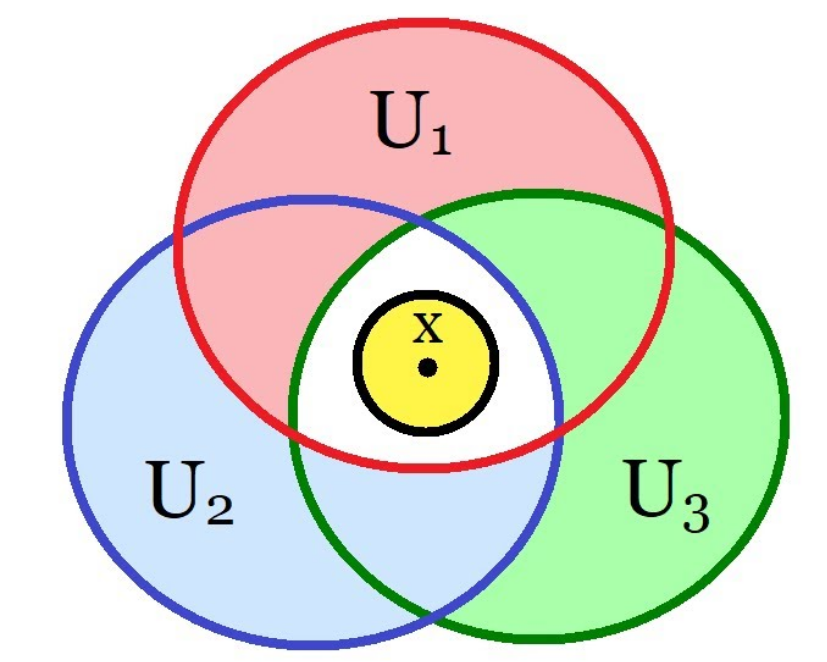
\includegraphics[width=0.35\textwidth]{pictures/baire.png}
\caption{Satz von Baire}
\end{figure}
\end{frame}

\begin{frame}
\frametitle{Satz von Baire}
\begin{dfi}[Mengenkategorisierung nach Baire]
\begin{itemize}
\item[(i)] $M \subset X$ \textit{nirgends dicht} in $X \Leftrightarrow (\bar{M})^\circ = \emptyset$
\item[(ii)] $M \subset X$ \textit{von 1.Kategorie} in $X \Leftrightarrow M = \bigcup\limits_{n \in \N}{\delta_n}$, $\delta_n$ nirgends dicht
\item[(iii)] $M \subset X$ \textit{von 2.Kategorie} in $X \Leftrightarrow M$ ist nicht von \textit{von 1.Kategorie}
\end{itemize}
\end{dfi}
\pause
\begin{sa}[Äquivalente Varianten des Satzes]
Folgende Aussagen sind äquivalent zu Satz \hyperref[sa_baire]{\ref*{sa_baire}}:
\begin{itemize}
\item[(ii)] Sei $(A_n)_{n \in \N}$ eine Folge von abgeschlossenen Teilmengen von $X$ mit leerem Inneren, so hat auch $\bigcup\limits_{n \in \N}{A_n}$ ein leeres Inneres. 
\item[(iii)] Jede offene nicht leere Teilmenge von $X$ ist von 2.Kategorie, d.h. sie lässt sich als eine abzählbare Vereinigung von nirgends dichten Teilmengen darstellen. Insbesondere ist $(X,d)$ in sich selbst von 2.Kategorie.
\end{itemize}
\end{sa}
\end{frame}

\begin{frame}
\frametitle{Satz von Baire}
\begin{block}{Anwendungsbeispiele}
\begin{itemize}
\item Der Satz von Baire ermöglicht elegante Beweise zentraler Sätze der klassischen Funktionalanalysis
\item Basis eines Banachraums
\item Existenz nirgends differenzierbarer Funktionen
\end{itemize}
\end{block}
\pause
\begin{sa}
Jede Basis eines unendlichdimensionalen Banachraumes ist überabzählbar.
\end{sa}
\end{frame}

\begin{frame}
\frametitle{Satz von Baire}
\begin{block}{Anwendungsbeispiel (Existenz nirgends differenzierbarer Funktionen)}
Auf $[0, 1]$ existieren stetige Funktionen, die an keiner Stelle differenzierbar sind. Wir setzen für $n \in \N$:
\begin{align*}
O_n := \left\{ f \in C[0,1] \bigg\vert \forall t \in [0,1]: \sup_{0<|h|<\frac{1}{n}}{\bigg\vert\frac{f(t+h)-f(t)}{h}\bigg\vert} > n \right\}
\end{align*}
Versieht man den Vektorraum $C[0,1]$ mit der Supremumsnorm, lässt sich zeigen, dass $O_n$ offen und dicht in $C[0,1]$ liegt.\\
\vspace{0.3cm}
$\overset{\text{Satz von Baire}}\Longrightarrow$ Der Raum $D := \bigcap\limits_{n \in \N}{O_n}$ liegt dicht in $C[0,1]$.\\
\vspace{0.3cm}
 Die Funktionen in $D$ sind stetig und an keiner Stelle differenzierbar.
\end{block}
\end{frame}

%%%%%%%%%%%%%%%%%%%%%%%%%%%%%%%%%
%Kompaktheit
%%%%%%%%%%%%%%%%%%%%%%%%%%%%%%%%%
\subsection{Kompaktheit}

\begin{frame}
\frametitle{Kompaktheit}
Im Folgenden sei $(X,d)$ ein metrischer Raum.
\pause
\begin{dfi}[Kompaktheit]
$K \subset X$ heißt \textit{kompakt}, falls jede offene Überdeckung 
\begin{align*}
K \subset \bigcup_{i \in I}{U_i} \enspace \text{mit} \enspace U_i \subset X
\end{align*}
eine endliche Teilüberdeckung
\begin{align*}
K \subset U_{i_1} \cup  U_{i_2} \cup \cdots \cup U_{i_n}  \enspace \text{mit} \enspace i_1, ..., i_n \in I
\end{align*}
besitzt.
\end{dfi}
\pause
\begin{dfi}[Folgenkompaktheit]
$K \subset X$ heißt \textit{folgenkompakt}, falls jede Folge in $K$ eine konvergente Teilfolge besitzt, die in $K$ konvergiert.
\end{dfi}
\end{frame}

\begin{frame}
\frametitle{Kompaktheit}
\begin{dfi}[Totalbeschränktheit]
$K \subset X$ heißt \textit{totalbeschränkt}, falls für alle $\epsilon > 0$ eine endliche Überdeckung mit offenen Kugeln existiert, d.h es existiert eine Menge von Punkten $x_1, ..., x_N \in K$ ($\epsilon$-Netz), so dass gilt:
\begin{align*} 
K \subset \bigcup_{n=1}^{N}{U_\epsilon(x_n)}
\end{align*} 
\end{dfi}
\pause
\begin{sa}
\label{komp_eq}
Für $K \subset X$ sind äquivalent:
\begin{itemize}
\item[(i)] $K$ ist kompakt
\item[(ii)] $K$ ist folgenkompakt
\item[(iii)] $K$ ist vollständig und totalbeschränkt
\end{itemize}
\end{sa}
\pause
(i) $\Leftrightarrow$ (iii) ist eine Verallgemeinerung des Satzes von Heine-Borel
\end{frame}

\begin{frame}
\frametitle{Kompaktheit}
Ist $(K,d)$ ein metrischer Raum und K kompakt, spricht man auch von einem \textit{kompakten Raum}.
\begin{figure}
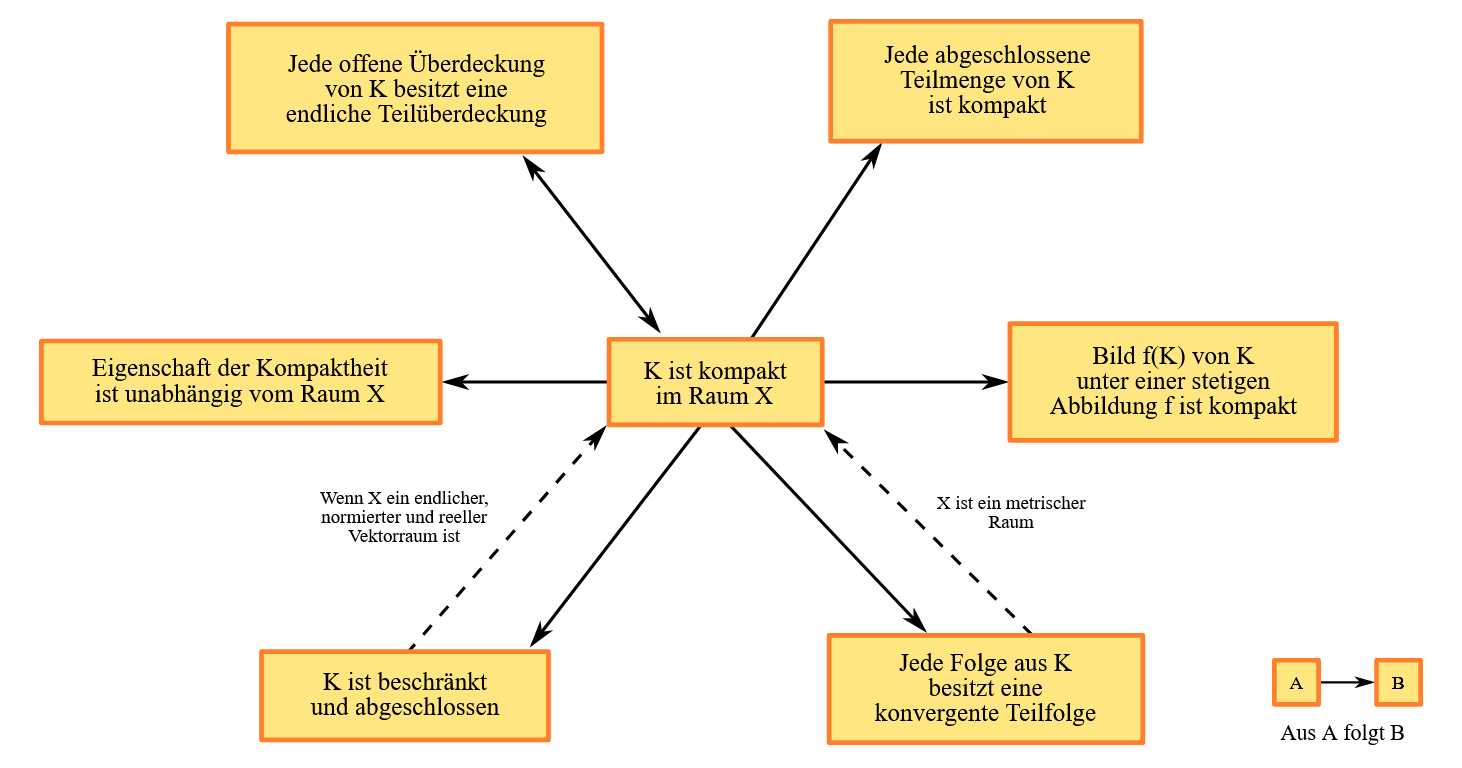
\includegraphics[width=0.92\textwidth]{pictures/kompaktheit.png}
\caption{Eigenschaften kompakter Mengen \cite{KompakterRaum}}
\end{figure}
\end{frame}

\begin{frame}
\frametitle{Kompaktheit}
\begin{lem}
Ist $K \subset X$ kompakt und $C \subset K$ abgeschlossen, dann ist auch C kompakt.
\end{lem}
\pause
\begin{lem}
(Ref \cite{Forster} Satz 2, S.38) Seien $a_v, b_v \in \R, a_v \leq b_v , v = 1, 2, . . . , n$. Dann ist der abgeschlossene Quader
$Q := \{(x_1, . . . , x_n) \in  \R^n : a_v \leq x_v \leq b_v \}$ kompakt in $\R^n$.


\end{lem}
\pause
\begin{lem}
(Ref. \cite{Clason}, Lemma 2.10) Ein kompakter metrischer Raum ist separabel.
\end{lem}
\pause
Die Umkehrung gilt allerdings nicht.\\
\textit{Beweis ...}
\end{frame}

%%%%%%%%%%%%%%%%%%%%%%%%%%%%%%%%%
%Satz von Heine Borel
%%%%%%%%%%%%%%%%%%%%%%%%%%%%%%%%%
\subsection{Satz von Heine Borel}

\begin{frame}
\frametitle{Satz von Heine Borel}
\begin{sa}[Satz von Heine-Borel]
\label{heine-borel}
$K \subset \R^n$ ist \textit{kompakt} $\Leftrightarrow$ K ist abgeschlossen und beschränkt
\end{sa}
\textit{Beweis ...}
\begin{figure}
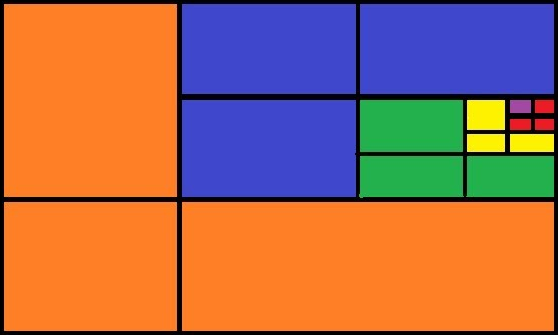
\includegraphics[width=0.35\textwidth]{pictures/heine-borel-theorem.png}
\caption{Boxen in Boxen in Boxen in Boxen...}
\end{figure}
\pause
\begin{block}{Schlechte Nachricht}
Ist der umgebene Raum jedoch unendlichdimensional dann gilt diese Äquivalenz nicht.
\end{block}
\end{frame}

\begin{frame}
\frametitle{Satz von Heine Borel}
Insbesondere ist mit Satz \hyperref[heine-borel]{\ref*{heine-borel}} die abgeschlossene Einheitskugel
\begin{align*}
B_1(x) = \{x \in \K^n | \|x\|_2 \leq 1\}
\end{align*}
 im euklidischen Raum kompakt.
Betrachten wir nun die abgeschlossene Einheitskugel im Banachraum $(C[0,1], \|\cdot\|_\infty)$:
\begin{align*}
B_1(x) = \{f \in C[0,1] \: | \: \|f\|_\infty \leq 1\}
\end{align*}
Es sei ${(f_k)}_{k \in \N}$ eine Folge von Funktionen $f_k \in (C[0,1], \|\cdot\|_\infty)$. Betrachten wir eine beliebige Teilfolge ${(f_{k_j})}_{j \in \N}$, dann gilt für beliebige $j \neq l$:
\begin{align*}
\|f_{k_j} - f_{k_l}\|_\infty = \max_{x \in [0,1]}{|f_{k_j}(x) - f_{k_l}(x)|} = 1
\end{align*}
Die Teilfolge ${(f_{k_j})}_{j \in \N}$ ist also keine Cauchy-Folge und besitzt damit keinen Grenzwert in $(C[0,1], \|\cdot\|_\infty)$. Damit ist die abgeschlossene Einheitskugel hier nicht kompakt.
\end{frame}

\begin{frame}
\frametitle{Satz von Heine Borel}
Für allgemeine metrische Räume gilt allerdings die Verallgemeinerung.
\pause
\begin{sa}[Verallgemeinerter Satz von Heine-Borel]
$K \subset X$ ist kompakt $\Leftrightarrow$ $K$ ist vollständig und totalbeschränkt
\end{sa}
\pause
Dies ist eine Verallgemeinerung, da für $A \subset \R^n$ gilt:
\begin{itemize}
\item $A$ ist vollständig $\Leftrightarrow$ $A$ ist abgeschlossen
\item $A$ ist totalbeschränkt $\Leftrightarrow$ $A$ ist beschränkt
\end{itemize}
\end{frame}

%%%%%%%%%%%%%%%%%%%%%%%%%%%%%%%%%
%Vollständigkeit der Folgen- und Funktionenräume
%%%%%%%%%%%%%%%%%%%%%%%%%%%%%%%%%
\subsection{Vollständigkeit der Folgen- und Funktionenräume}

\begin{frame}
\frametitle{Vollständigkeit der Folgen- und Funktionenräume}
\begin{dfi}[Der Funktionenraum]
Sei $D$ eine nichtleere Menge und $X$ ein Vektorraum über $\K$, dann bezeichnet $Abb(D,X)$ die Menge aller Funktionen von $D$ nach $X$:
\begin{align*}
Abb(D,X) := \{f \: | \: f : D \rightarrow X\}
\end{align*}
Ist die Menge bezüglich der Addition und Skalarmultiplikation abgeschlossen, spricht man von einem linearen Funktionenraum:
\begin{itemize}
\item[(i)]  $+ : Abb(D,X) \times Abb(D,X) \rightarrow Abb(D,X), (f + g)(x) = f(x) + g(x)$\\
\item[(ii)]  $\cdot :  \K \times Abb(D,X) \rightarrow Abb(D,X), (\lambda f)g(x) = \lambda f(x)$\\
\end{itemize}
\end{dfi}
\pause
\begin{bsp}
Menge aller stetigen Funktionen auf dem Intervall $[a,b] \subset \R$:
\begin{align*}
C[a,b] := \left\{ f : [a,b] \rightarrow \K \: | \: f \: \text{ist stetig} \right\}
\end{align*}
\end{bsp}
\end{frame}

\begin{frame}
\frametitle{Vollständigkeit der Folgen- und Funktionenräume}
\begin{sa}
$(C[a,b], \|\cdot\|_\infty)$ ist ein Banachraum.
\end{sa}
\textit{Beweis...}
\end{frame}

\begin{frame}
\frametitle{Vollständigkeit der Folgen- und Funktionenräume}
\begin{dfi}[Der Folgenraum]
Wir nennen die Menge aller Folgen über $\K$ den Folgenraum:
\begin{align*}
\K^\N := \{{(x_k)}_{k \in \N} : x_k \in \K \: \text{für} \: \forall k \in \N\}
\end{align*}
Auf  $\K^\N$ sind auch wieder folgende Vektorraumverknüpfungen definiert:
\begin{itemize}
\item[(i)]  $+ \K^\N \times \K^\N \rightarrow \K^\N, {(x_k)}_{k \in \N} + {(y_k)}_{k \in \N} := (x_k + y_k)_{k \in \N}$\\
\item[(ii)] $\cdot : \K \times \K^\N \rightarrow \K^\N, \lambda{(x_k)}_{k \in \N} := {(\lambda x_k)}_{k \in \N}$\\
\end{itemize}
\end{dfi}
\pause
\begin{bsp}
Wir definieren uns Teilmengen (hier sogar Unterräume) des Folgenraums:
\begin{align*}
\ell^\infty(\K) := &\left\{x \in \K^\N : x = {(x_k)}_{k \in \N} \: \text{ist beschränkt} \right\},\\
c(\K) := &\left\{x \in \K^\N : x = {(x_k)}_{k \in \N} \: \text{ist konvergent} \right\}
\end{align*}
\end{bsp}
\end{frame}

\begin{frame}
\frametitle{Vollständigkeit der Folgen- und Funktionenräume}
\begin{sa}
Der Raum $(\ell^\infty(\K), \|\cdot\|_\infty)$ ist ein Banachraum.
\end{sa}
\end{frame}

%%%%%%%%%%%%%%%%%%%%%%%%%%%%%%%%%%%%%%%%%%%%%%%%%%%%%%%%%%%%%%%%%%
%Abbildungsverzeichnis
%%%%%%%%%%%%%%%%%%%%%%%%%%%%%%%%%%%%%%%%%%%%%%%%%%%%%%%%%%%%%%%%%%
\section{Abbildungsverzeichnis}

\begin{frame}
\frametitle{Abbildungsverzeichnis}
\printbibliography[heading=none, nottype=article, nottype=book]
\end{frame}

%%%%%%%%%%%%%%%%%%%%%%%%%%%%%%%%%%%%%%%%%%%%%%%%%%%%%%%%%%%%%%%%%%
%Literatur
%%%%%%%%%%%%%%%%%%%%%%%%%%%%%%%%%%%%%%%%%%%%%%%%%%%%%%%%%%%%%%%%%%
\section{Literatur}

\begin{frame}
\frametitle{Literatur}
\printbibliography[heading=none, type=book]
\end{frame}

%%%%%%%%%%%%%%%%%%%%%%%%%%%%%%%%%%%%%%%%%%%%%%%%%%%%%%%%%%%%%%%%%%
%Danke
%%%%%%%%%%%%%%%%%%%%%%%%%%%%%%%%%%%%%%%%%%%%%%%%%%%%%%%%%%%%%%%%%%
\begin{frame}
\frametitle{Danke}

{\large \glqq Mathematik ist die schönste und mächtigste Schöpfung des menschlichen Geistes.\grqq \: -\:  Stefan Banach \par}
\vspace{0.5cm}
\pause
%\begin{center}
%{\Large Danke für eure Aufmerksamheit! \par}
%\end{center}

\centering
\begin{figure}

\includegraphics[width=0.7\textwidth]{pictures/leonardo-meme.png}
\caption{Leonardo DiCaprio als Jay Gatsby in The Great Gatsby \cite{LeonardoMeme}}
\end{figure}

\end{frame}

\end{document}